% Options for packages loaded elsewhere
\PassOptionsToPackage{unicode}{hyperref}
\PassOptionsToPackage{hyphens}{url}
\PassOptionsToPackage{dvipsnames,svgnames,x11names}{xcolor}
%
\documentclass[
  10pt,
]{article}
\usepackage{amsmath,amssymb}
\usepackage{iftex}
\ifPDFTeX
  \usepackage[T1]{fontenc}
  \usepackage[utf8]{inputenc}
  \usepackage{textcomp} % provide euro and other symbols
\else % if luatex or xetex
  \usepackage{unicode-math} % this also loads fontspec
  \defaultfontfeatures{Scale=MatchLowercase}
  \defaultfontfeatures[\rmfamily]{Ligatures=TeX,Scale=1}
\fi
\usepackage{lmodern}
\ifPDFTeX\else
  % xetex/luatex font selection
  \setmainfont[]{DejaVu Sans}
  \setmonofont[]{DejaVu Sans Mono}
  \setmathfont[]{DejaVu Sans}
\fi
% Use upquote if available, for straight quotes in verbatim environments
\IfFileExists{upquote.sty}{\usepackage{upquote}}{}
\IfFileExists{microtype.sty}{% use microtype if available
  \usepackage[]{microtype}
  \UseMicrotypeSet[protrusion]{basicmath} % disable protrusion for tt fonts
}{}
\makeatletter
\@ifundefined{KOMAClassName}{% if non-KOMA class
  \IfFileExists{parskip.sty}{%
    \usepackage{parskip}
  }{% else
    \setlength{\parindent}{0pt}
    \setlength{\parskip}{6pt plus 2pt minus 1pt}}
}{% if KOMA class
  \KOMAoptions{parskip=half}}
\makeatother
\usepackage{xcolor}
\usepackage[margin=2.2cm]{geometry}
\usepackage{longtable,booktabs,array}
\usepackage{calc} % for calculating minipage widths
% Correct order of tables after \paragraph or \subparagraph
\usepackage{etoolbox}
\makeatletter
\patchcmd\longtable{\par}{\if@noskipsec\mbox{}\fi\par}{}{}
\makeatother
% Allow footnotes in longtable head/foot
\IfFileExists{footnotehyper.sty}{\usepackage{footnotehyper}}{\usepackage{footnote}}
\makesavenoteenv{longtable}
\usepackage{graphicx}
\makeatletter
\def\maxwidth{\ifdim\Gin@nat@width>\linewidth\linewidth\else\Gin@nat@width\fi}
\def\maxheight{\ifdim\Gin@nat@height>\textheight\textheight\else\Gin@nat@height\fi}
\makeatother
% Scale images if necessary, so that they will not overflow the page
% margins by default, and it is still possible to overwrite the defaults
% using explicit options in \includegraphics[width, height, ...]{}
\setkeys{Gin}{width=\maxwidth,height=\maxheight,keepaspectratio}
% Set default figure placement to htbp
\makeatletter
\def\fps@figure{htbp}
\makeatother
\setlength{\emergencystretch}{3em} % prevent overfull lines
\providecommand{\tightlist}{%
  \setlength{\itemsep}{0pt}\setlength{\parskip}{0pt}}
\setcounter{secnumdepth}{-\maxdimen} % remove section numbering

\usepackage{xcolor}
\definecolor{plblue}{HTML}{1F3864}
\usepackage{sectsty}
\allsectionsfont{\sffamily\color{plblue}}
\usepackage{fvextra}
\DefineVerbatimEnvironment{Highlighting}{Verbatim}{breaklines,commandchars=\\\{\},fontsize=\footnotesize}
\usepackage{etoolbox}
\AtBeginEnvironment{longtable}{\footnotesize}
\ifLuaTeX
  \usepackage{selnolig}  % disable illegal ligatures
\fi
\IfFileExists{bookmark.sty}{\usepackage{bookmark}}{\usepackage{hyperref}}
\IfFileExists{xurl.sty}{\usepackage{xurl}}{} % add URL line breaks if available
\urlstyle{same}
\hypersetup{
  colorlinks=true,
  linkcolor={Maroon},
  filecolor={Maroon},
  citecolor={Blue},
  urlcolor={Blue},
  pdfcreator={LaTeX via pandoc}}

\author{}
\date{}

\begin{document}

\hypertarget{document-3-tests}{%
\section{Document 3: Tests}\label{document-3-tests}}

\textbf{Kit:} qae\_european 1.0.0 · \textbf{Status of this document:}
Part 1 (test plan) frozen by its commit before the campaign (422ebfb);
Part 2 (results) written after the campaign. Sign-off of the whole kit
by Romain Dutrenois at the end, after an independent review.

Part 1 is pre-registered: it is written and committed \textbf{before}
the campaign runs, and the commit date is the proof. Any change made
after that commit is recorded in the deviations table (section 1.9),
with its reason.

\begin{center}\rule{0.5\linewidth}{0.5pt}\end{center}

\hypertarget{part-1-test-plan}{%
\subsection{Part 1: Test plan}\label{part-1-test-plan}}

\hypertarget{11-what-we-want-to-test-and-why}{%
\subsubsection{1.1 What we want to test, and
why}\label{11-what-we-want-to-test-and-why}}

The kit prices a European call with \textbf{maximum-likelihood amplitude
estimation} (MLAE) on a quantum circuit simulator. The claim to test is
the theoretical promise of amplitude estimation: \textbf{it needs fewer
samples than Monte Carlo to reach the same accuracy}, quadratically
fewer in the limit.

\textbf{Measure of performance: relative efficiency in number of calls.}
Performance is measured by the error reached for a given number of calls
(sample complexity, or \emph{query complexity} for amplitude estimation,
where a call is a query to the circuit A). Two methods are compared
through their \textbf{relative efficiency} at a given RMSE ε:

E(ε) = N\_comparator(ε) / N\_QAE(ε)

where N(ε) is the number of calls a method needs to reach RMSE ε. E
\textgreater{} 1 means amplitude estimation needs fewer calls than the
comparator; E \textless{} 1 means it needs more. Calls are counted as
follows:

\begin{itemize}
\tightlist
\item
  For amplitude estimation, a call is one application of the circuit A.
  One Grover step contains A and its inverse, so a measurement after k
  Grover steps counts as 2k + 1 calls.
\item
  For Monte Carlo, a call is one simulated path, i.e. one payoff
  evaluation.
\item
  For quasi-Monte Carlo, a call is one point of the Sobol sequence.
\end{itemize}

\textbf{Out of scope:}

\begin{itemize}
\tightlist
\item
  \textbf{Speed (wall-clock time).} The campaign runs on a classical
  simulator, which is far slower than Monte Carlo. No current quantum
  machine can run the deeper circuits usefully. Speed is discussed only
  as a projection from published resource estimates, labelled as such.
\item
  \textbf{Hardware noise.} The simulator is noise-free. No run on a real
  machine in this campaign.
\end{itemize}

\textbf{Accuracy is decomposed.} The circuit prices the option on a grid
of 2ⁿ points, not on the continuous distribution. Its error against
Black-Scholes therefore has two parts, measured separately:

\begin{itemize}
\tightlist
\item
  \textbf{discretisation bias} = grid price − Black-Scholes price
  (deterministic, depends on n);
\item
  \textbf{statistical error} = estimate − grid price (random, depends on
  the number of calls).
\end{itemize}

\hypertarget{12-hypotheses}{%
\subsubsection{1.2 Hypotheses}\label{12-hypotheses}}

\begin{longtable}[]{@{}
  >{\raggedright\arraybackslash}p{(\columnwidth - 4\tabcolsep) * \real{0.0933}}
  >{\raggedright\arraybackslash}p{(\columnwidth - 4\tabcolsep) * \real{0.5735}}
  >{\raggedright\arraybackslash}p{(\columnwidth - 4\tabcolsep) * \real{0.3131}}@{}}
\toprule\noalign{}
\begin{minipage}[b]{\linewidth}\raggedright
\#
\end{minipage} & \begin{minipage}[b]{\linewidth}\raggedright
Hypothesis
\end{minipage} & \begin{minipage}[b]{\linewidth}\raggedright
Type
\end{minipage} \\
\midrule\noalign{}
\endhead
\bottomrule\noalign{}
\endlastfoot
H0 & The circuit computes the grid price exactly, and the identity used
to accelerate the campaign holds. & Prerequisite \\
H1 & At equal calls, the RMSE of amplitude estimation is below that of
plain Monte Carlo sampling the same grid, i.e. a relative efficiency E
\textgreater{} 1. & Relative efficiency against plain Monte Carlo \\
H2 & The query complexity of amplitude estimation is O(1/ε), against
O(1/ε²) for plain Monte Carlo: its statistical error falls like 1/N,
against 1/√N. & Query complexity (convergence rate) \\
H3 & With 7 price qubits and the largest budget, the total error against
Black-Scholes is within tolerance. & Accuracy against the reference \\
H4 & Against quasi-Monte Carlo, the best classical sampling method for
this one-dimensional problem, no relative efficiency above 1 is
expected. & Descriptive: measured, no pass/fail \\
\end{longtable}

H4 is stated in advance as an expected \textbf{absence} of gain (E ≤ 1).
Quasi-Monte Carlo converges close to 1/N on smooth one-dimensional
problems, the same rate as amplitude estimation.

\hypertarget{13-methods-compared}{%
\subsubsection{1.3 Methods compared}\label{13-methods-compared}}

\begin{longtable}[]{@{}
  >{\raggedright\arraybackslash}p{(\columnwidth - 4\tabcolsep) * \real{0.3893}}
  >{\raggedright\arraybackslash}p{(\columnwidth - 4\tabcolsep) * \real{0.2271}}
  >{\raggedright\arraybackslash}p{(\columnwidth - 4\tabcolsep) * \real{0.3636}}@{}}
\toprule\noalign{}
\begin{minipage}[b]{\linewidth}\raggedright
Method
\end{minipage} & \begin{minipage}[b]{\linewidth}\raggedright
Target
\end{minipage} & \begin{minipage}[b]{\linewidth}\raggedright
Role
\end{minipage} \\
\midrule\noalign{}
\endhead
\bottomrule\noalign{}
\endlastfoot
Black-Scholes closed form & Continuous price & Reference ("truth") \\
Exact circuit probability & Grid price & Checks the circuit (H0) \\
Amplitude estimation (MLAE) & Grid price & Method under test \\
Plain Monte Carlo on the grid & Grid price & Like-for-like comparator
for H1, H2 \\
Plain Monte Carlo, continuous & Continuous price & What a desk would see
with plain sampling \\
Quasi-Monte Carlo (scrambled Sobol), continuous & Continuous price &
Best classical sampling method (H4) \\
\end{longtable}

Methods and code are described in Document 2 (Benchmarks).

\hypertarget{14-scenario-grid}{%
\subsubsection{1.4 Scenario grid}\label{14-scenario-grid}}

Spot fixed at 100. All combinations of:

\begin{longtable}[]{@{}
  >{\raggedright\arraybackslash}p{(\columnwidth - 4\tabcolsep) * \real{0.3478}}
  >{\raggedright\arraybackslash}p{(\columnwidth - 4\tabcolsep) * \real{0.4490}}
  >{\raggedright\arraybackslash}p{(\columnwidth - 4\tabcolsep) * \real{0.1833}}@{}}
\toprule\noalign{}
\begin{minipage}[b]{\linewidth}\raggedright
Dimension
\end{minipage} & \begin{minipage}[b]{\linewidth}\raggedright
Values
\end{minipage} & \begin{minipage}[b]{\linewidth}\raggedright
Count
\end{minipage} \\
\midrule\noalign{}
\endhead
\bottomrule\noalign{}
\endlastfoot
Moneyness K / S₀ & 0.75 to 1.25, step 0.05 & 11 \\
Maturity & 1W, 2W, 1M, 3M, 6M, 1Y, 3Y, 5Y & 8 \\
Volatility & 20\% to 80\%, step 10\% & 7 \\
Rate & −1\%, 0\%, +1\% & 3 \\
\end{longtable}

That is \textbf{1,848 scenarios}. Each is crossed with:

\begin{itemize}
\tightlist
\item
  \textbf{price qubits} n = 3, 4, 5, 6, 7 (grids of 8 to 128 points);
\item
  \textbf{5 budgets}: MLAE ladders of depth 4 to 8, i.e. Grover powers
  (0, 1, 2, 4, \ldots, 2\^{}(depth−2)), 100 measurements per power. That
  gives 1,800, 3,500, 6,800, 13,300 and 26,200 calls. Monte Carlo
  methods get the same number of calls; quasi-Monte Carlo uses the
  largest power of two not above it;
\item
  \textbf{50 independent draws} of every random method.
\end{itemize}

In total: 1,848 × 5 × 5 = 46,200 configurations, about 9.2 million
priced estimates. \emph{{[}Erratum, see 1.9: 2.31 million
amplitude-estimation estimates, about 5.5 million in all.{]}}

\hypertarget{15-measured-quantities}{%
\subsubsection{1.5 Measured quantities}\label{15-measured-quantities}}

For each scenario, number of qubits n and budget N, the campaign stores:

\begin{itemize}
\tightlist
\item
  the Black-Scholes price, the grid price and the exact circuit price;
\item
  for each random method, the \textbf{root-mean-square error (RMSE)}
  over the 50 draws, against its own target (grid price or
  Black-Scholes, as in 1.3), and the RMSE of amplitude estimation
  against Black-Scholes;
\item
  for amplitude estimation and Monte Carlo on the grid, the
  \textbf{median absolute error} against the grid price, which is not
  driven by a few large errors;
\item
  for amplitude estimation, the \textbf{share of mode errors}: draws
  where the estimated θ is further than π / (2 m\_max) from the true θ,
  with m\_max = 2 k\_max + 1 the multiplier of the highest Grover power.
  That is half the period of the most informative measurement, so such a
  draw has locked onto a wrong peak of the likelihood;
\item
  the number of calls actually used.
\end{itemize}

Seeds are derived from a fixed master seed (20261103) and the indices of
scenario, qubits, budget and method, so any row can be recomputed on its
own.

\hypertarget{16-scope-rules-decided-before-the-run}{%
\subsubsection{1.6 Scope rules: decided before the
run}\label{16-scope-rules-decided-before-the-run}}

\begin{itemize}
\tightlist
\item
  \textbf{Out-of-grid scenarios.} When every grid point is out of the
  money, the circuit price is exactly 0 and there is nothing to
  estimate. These are counted and reported, and excluded from H1 to H4.
\item
  \textbf{Negligible prices.} Scenarios with a Black-Scholes price below
  0.01 (one cent on a spot of 100) are reported separately and excluded
  from H1 to H4. Relative errors are meaningless there.
\item
  \textbf{Everything else is in scope.} No scenario is excluded after
  the results are seen.
\end{itemize}

\hypertarget{17-acceptance-criteria}{%
\subsubsection{1.7 Acceptance criteria}\label{17-acceptance-criteria}}

\begin{longtable}[]{@{}
  >{\raggedright\arraybackslash}p{(\columnwidth - 4\tabcolsep) * \real{0.0881}}
  >{\raggedright\arraybackslash}p{(\columnwidth - 4\tabcolsep) * \real{0.5341}}
  >{\raggedright\arraybackslash}p{(\columnwidth - 4\tabcolsep) * \real{0.3578}}@{}}
\toprule\noalign{}
\begin{minipage}[b]{\linewidth}\raggedright
\#
\end{minipage} & \begin{minipage}[b]{\linewidth}\raggedright
Criterion
\end{minipage} & \begin{minipage}[b]{\linewidth}\raggedright
Pass if
\end{minipage} \\
\midrule\noalign{}
\endhead
\bottomrule\noalign{}
\endlastfoot
H0-a & Circuit price against grid price, every scenario and every n &
Absolute difference ≤ 1e-9 in \textbf{100\%} of cases \\
H0-b & Full statevector simulation of A Qᵏ against sin²((2k + 1)θ), on
20 randomly drawn scenarios (powers up to 64 for n ≤ 5, up to 8 for n =
6, 7) & Absolute difference ≤ 1e-9 in \textbf{100\%} of checks \\
H1 & At the largest budget (26,200 calls), RMSE of amplitude estimation
\textless{} RMSE of Monte Carlo on the same grid & In \textbf{≥ 95\%} of
in-scope (scenario, n) pairs \\
H2-a & Fitted slope of log RMSE against log N over the 5 budgets,
amplitude estimation, n = 5 & Slope ≤ −0.8 in \textbf{≥ 90\%} of
in-scope scenarios \\
H2-b & Same fit for Monte Carlo on the grid (checks the benchmark) &
Slope between −0.65 and −0.35 in \textbf{≥ 90\%} of in-scope
scenarios \\
H3 & n = 7, largest budget: RMSE of amplitude estimation against
Black-Scholes ≤ max(1\% of the Black-Scholes price, 0.01) & In \textbf{≥
95\%} of in-scope scenarios \\
H4 & Ratio of RMSE against Black-Scholes, amplitude estimation (n = 7)
over quasi-Monte Carlo, at each budget & Descriptive: distribution
reported, no pass/fail \\
\end{longtable}

\textbf{Verdict per hypothesis:} \emph{Validated} if the criterion
passes; \emph{Not validated} otherwise. If a criterion fails only in an
identifiable region of the grid (for example very short maturities), the
verdict is \emph{Validated with limits}, naming that region. Failure of
H0 stops the campaign: nothing else is interpreted.

\hypertarget{18-reported-analyses-in-addition-to-the-criteria}{%
\subsubsection{1.8 Reported analyses (in addition to the
criteria)}\label{18-reported-analyses-in-addition-to-the-criteria}}

\begin{itemize}
\tightlist
\item
  \textbf{Relative efficiency E at the largest budget}, per in-scope
  scenario, against Monte Carlo on the grid (n = 5 and n = 7) and
  against quasi-Monte Carlo (n = 7): median, first and third quartiles.
  E is estimated from the fitted error curves: E = N\_comparator(ε) /
  N\_QAE(ε), with ε the RMSE of amplitude estimation at its largest
  budget, and N\_comparator(ε) read from the
  comparator\textquotesingle s fitted log RMSE against log N
  (extrapolated beyond 26,200 calls where needed, flagged as such).
\item
  Errors by dimension: moneyness, maturity, volatility, rate and number
  of qubits, to find where amplitude estimation works best and worst.
\item
  The crossing budget N*: the smallest budget where amplitude estimation
  beats Monte Carlo on the grid, for each scenario.
\item
  Discretisation bias against Black-Scholes, as a function of n and of
  the scenario.
\item
  The hard cases: deep out-of-the-money options (small amplitude), very
  short maturities, high volatility.
\item
  Counts of out-of-grid and negligible-price scenarios.
\item
  \textbf{Mode errors of amplitude estimation}: their share by scenario,
  number of qubits and budget, and where they concentrate. H1 is also
  reported on the median absolute error, as a sensitivity check. The
  criterion itself stays on the RMSE.
\end{itemize}

\hypertarget{19-deviations-from-the-plan}{%
\subsubsection{1.9 Deviations from the
plan}\label{19-deviations-from-the-plan}}

\begin{longtable}[]{@{}
  >{\raggedright\arraybackslash}p{(\columnwidth - 6\tabcolsep) * \real{0.0460}}
  >{\raggedright\arraybackslash}p{(\columnwidth - 6\tabcolsep) * \real{0.4567}}
  >{\raggedright\arraybackslash}p{(\columnwidth - 6\tabcolsep) * \real{0.3853}}
  >{\raggedright\arraybackslash}p{(\columnwidth - 6\tabcolsep) * \real{0.0920}}@{}}
\toprule\noalign{}
\begin{minipage}[b]{\linewidth}\raggedright
Date
\end{minipage} & \begin{minipage}[b]{\linewidth}\raggedright
Deviation
\end{minipage} & \begin{minipage}[b]{\linewidth}\raggedright
Reason
\end{minipage} & \begin{minipage}[b]{\linewidth}\raggedright
Approved by
\end{minipage} \\
\midrule\noalign{}
\endhead
\bottomrule\noalign{}
\endlastfoot
2026-11-10 & \textbf{Corrections after an internal review, and the
campaign re-run.} A review in a separate session, working from a fresh
clone, found that the MLAE maximisation refined only the best grid
point, so with two nearly tied likelihood peaks it could return the
lower one (1 draw in 2.31 million in the first campaign; frequent at
depths above 8). Corrected: denser grid for deep ladders, and refinement
of the 5 highest grid peaks (Document 1, section 6). Because the code
that produced the results changed, \textbf{the whole campaign was
re-run} on the corrected code (commit 2d83462). At the same time, and
before the re-run: H0-b was extended with the full ladder (powers up to
64) at n = 6 and 7 on one scenario; the campaign resume refuses
incomplete scenarios; \texttt{run\_info.json} became a log of every run;
\texttt{docs/analyse.py} and \texttt{docs/checks.py} were extended so
every number in Part 2 is computed by a script. Criteria unchanged. The
first campaign\textquotesingle s results stay in the repository history
(commit 373e6a1). & Optimiser error and traceability gaps found in
review & Developer (Veqctor) \\
2026-11-10 & \textbf{Erratum to 1.4.} "About 9.2 million priced
estimates" counted continuous Monte Carlo and quasi-Monte Carlo once per
number of qubits. They are computed once per scenario and budget: 2.31
million amplitude-estimation estimates, about 5.5 million in all. &
Counting error in the plan text & Developer (Veqctor) \\
2026-11-10 & \textbf{Proposed, not applied: H0-a restated as a relative
tolerance}, \textbar circuit − grid\textbar{} ≤ 1e-8 × grid price. Post
hoc: made after seeing that H0-a fails as written (Part 2, section 2.4).
& The absolute tolerance of 1e-9 did not allow for the floating-point
error of Qiskit\textquotesingle s state-preparation synthesis at 6 and 7
qubits (relative error up to 3.4e-9) & Pending: independent review and
sign-off \\
2026-11-10 & \textbf{First campaign run discarded, unread.} It ran on a
stale installed copy of the package (20 draws, without the measures
added above). Detected when the analysis script stopped on the missing
columns, before computing any statistic. The run was moved aside without
being analysed; the package was reinstalled in editable mode; the
analysis script (\texttt{docs/analyse.py}) was committed before the
rerun; each run now writes \texttt{results/run\_info.json} (git commit,
draws, versions) next to its results. & Execution error, recorded for
transparency & Developer (Veqctor) \\
2026-11-10 & \textbf{Draws raised from 20 to 50; median absolute error
and share of mode errors added to the stored measures (1.5) and reported
analyses (1.8).} Criteria unchanged. & While writing the user guide, one
scenario was recomputed (scenario 1000: at the money, 5Y, vol 60\%, rate
0\%; n = 5, largest budget). One of its 20 draws had locked onto a wrong
peak of the likelihood (θ off by about π/129), giving a price error of
33 on a price of 49; the RMSE over 20 draws was 7.4, against 0.5 over
200 draws. This is a known property of maximum-likelihood amplitude
estimation: errors are mostly small, with rare large ones. With 20 draws
the RMSE would depend on whether such a draw is in the sample. The
method itself is left unchanged (the published one); the measurement is
made more stable and the rare errors are counted rather than hidden. No
other scenario was inspected. & Developer (Veqctor) \\
2026-11-03 & Terminology: "superiority" replaced by \textbf{relative
efficiency} and \textbf{query complexity} (sections 1.1, 1.2), and the
distribution of E added to the reported analyses (1.8). Criteria and
thresholds unchanged. Made before any run. & Standard statistical terms,
measurable per scenario & Romain Dutrenois \\
2026-11-03 & Before this campaign, in the exploratory version of the
kit, the amplitude-estimation tolerance was tightened from 2\% to 1\%
after a first run, and the budget increased. This plan replaces those
exploratory tests; its criteria are set without reference to them. &
Recorded for transparency & --- \\
\end{longtable}

\hypertarget{110-execution}{%
\subsubsection{1.10 Execution}\label{110-execution}}

\begin{itemize}
\tightlist
\item
  \textbf{Environment:} Python 3.13, Qiskit 2.6.1, NumPy 2.5.4, SciPy
  1.18.1, all versions pinned in \texttt{requirements-lock.txt}. CPU:
  2-core Intel Xeon at 2.8 GHz, Linux. Details in Document 1.
\item
  \textbf{Commands:} \texttt{qae-european\ verify} (H0-b), then
  \texttt{qae-european\ campaign\ -\/-processes\ 2} (resumable). Output:
  \texttt{results/verification.json}, \texttt{results/campaign.csv} and
  \texttt{results/run\_info.json} (the git commit, parameters and
  library versions of the run). The analysis against the criteria is
  \texttt{docs/analyse.py}, committed before the run.
\item
  \textbf{Acceleration (declared).} In the campaign,
  amplitude-estimation measurements are drawn from the exact
  probabilities sin²((2k + 1)θ), with θ taken from the exact statevector
  of the circuit A for each scenario. On a noise-free simulator, this is
  mathematically identical to simulating the circuits A Qᵏ. The identity
  is verified by H0-b.
\item
  \textbf{Sizing.} Timing was measured on 3 scenarios, timing only,
  without inspecting results: about 1.5 s per scenario with 20 draws, so
  about 25 minutes in total. With 50 draws: about 1 hour on 2 cores.
\end{itemize}

\hypertarget{111-sign-off}{%
\subsubsection{1.11 Sign-off}\label{111-sign-off}}

\begin{longtable}[]{@{}
  >{\raggedright\arraybackslash}p{(\columnwidth - 6\tabcolsep) * \real{0.2116}}
  >{\raggedright\arraybackslash}p{(\columnwidth - 6\tabcolsep) * \real{0.3664}}
  >{\raggedright\arraybackslash}p{(\columnwidth - 6\tabcolsep) * \real{0.2443}}
  >{\raggedright\arraybackslash}p{(\columnwidth - 6\tabcolsep) * \real{0.1577}}@{}}
\toprule\noalign{}
\begin{minipage}[b]{\linewidth}\raggedright
Role
\end{minipage} & \begin{minipage}[b]{\linewidth}\raggedright
Name
\end{minipage} & \begin{minipage}[b]{\linewidth}\raggedright
Decision
\end{minipage} & \begin{minipage}[b]{\linewidth}\raggedright
Date
\end{minipage} \\
\midrule\noalign{}
\endhead
\bottomrule\noalign{}
\endlastfoot
Author & Veqctor (kit generation) & Submitted & 2026-11-03 \\
Internal review & Developer\textquotesingle s reviewer (separate
session, fresh clone) & Findings corrected (1.9) & 2026-11-10 \\
Independent review & AI reviewer (separate project, no access to the
build) & & \\
Sign-off & Romain Dutrenois & & \\
\end{longtable}

\begin{center}\rule{0.5\linewidth}{0.5pt}\end{center}

\hypertarget{part-2-results}{%
\subsection{Part 2: Results}\label{part-2-results}}

Every number below is computed by a script in the kit:

\begin{itemize}
\tightlist
\item
  \texttt{docs/analyse.py} writes \texttt{results/summary.json} from
  \texttt{results/campaign.csv} and \texttt{results/verification.json}.
\item
  \texttt{docs/checks.py} writes \texttt{results/checks.json}: the
  state-preparation accuracy and the global-maximum check of MLAE.
\end{itemize}

All of these files are in the repository. Where the text quotes a
number, the key in the JSON file is given in brackets.

\hypertarget{21-execution-record}{%
\subsubsection{2.1 Execution record}\label{21-execution-record}}

\begin{longtable}[]{@{}
  >{\raggedright\arraybackslash}p{(\columnwidth - 2\tabcolsep) * \real{0.2315}}
  >{\raggedright\arraybackslash}p{(\columnwidth - 2\tabcolsep) * \real{0.7485}}@{}}
\toprule\noalign{}
\begin{minipage}[b]{\linewidth}\raggedright
Item
\end{minipage} & \begin{minipage}[b]{\linewidth}\raggedright
Value
\end{minipage} \\
\midrule\noalign{}
\endhead
\bottomrule\noalign{}
\endlastfoot
Code & commit 2d83462, no uncommitted changes in the package
(\texttt{results/run\_info.json}) \\
Plan & frozen at commit 422ebfb; criteria unchanged since \\
Environment & Python 3.13.17, Qiskit 2.6.1, NumPy 2.5.4, SciPy 1.18.1,
Linux, 2 cores \\
Run & 2026-11-10: verification (100 checks), then 1,848 scenarios × 5
qubit counts × 5 budgets × 50 draws, in one call \\
Rows & 46,200 (complete) \\
Wall time & about 12 minutes for the verification and 25 minutes for the
campaign, on 2 cores \\
\end{longtable}

\textbf{Runs before this one} (section 1.9):

\begin{enumerate}
\def\labelenumi{\arabic{enumi}.}
\tightlist
\item
  \textbf{A first run was discarded unread.} It ran on a stale copy of
  the package.
\item
  \textbf{A second run was complete and published} (commit 373e6a1). An
  internal review then found the MLAE optimiser could return the lower
  of two nearly tied peaks. The optimiser was corrected and the campaign
  re-run. That is this run.
\end{enumerate}

Its results differ from the second run\textquotesingle s in a handful of
configurations:

\begin{longtable}[]{@{}
  >{\raggedright\arraybackslash}p{(\columnwidth - 4\tabcolsep) * \real{0.3924}}
  >{\raggedright\arraybackslash}p{(\columnwidth - 4\tabcolsep) * \real{0.3102}}
  >{\raggedright\arraybackslash}p{(\columnwidth - 4\tabcolsep) * \real{0.2774}}@{}}
\toprule\noalign{}
\begin{minipage}[b]{\linewidth}\raggedright
Statistic
\end{minipage} & \begin{minipage}[b]{\linewidth}\raggedright
Second run
\end{minipage} & \begin{minipage}[b]{\linewidth}\raggedright
This run
\end{minipage} \\
\midrule\noalign{}
\endhead
\bottomrule\noalign{}
\endlastfoot
H1 passes & 8,772 & 8,774 \\
H3 passes & 1,594 & 1,595 \\
Mode-error draws & 45 & 44 \\
\end{longtable}

No verdict changes.

\hypertarget{22-scope}{%
\subsubsection{2.2 Scope}\label{22-scope}}

\begin{longtable}[]{@{}
  >{\raggedright\arraybackslash}p{(\columnwidth - 4\tabcolsep) * \real{0.3115}}
  >{\raggedright\arraybackslash}p{(\columnwidth - 4\tabcolsep) * \real{0.2910}}
  >{\raggedright\arraybackslash}p{(\columnwidth - 4\tabcolsep) * \real{0.3775}}@{}}
\toprule\noalign{}
\begin{minipage}[b]{\linewidth}\raggedright
Category
\end{minipage} & \begin{minipage}[b]{\linewidth}\raggedright
Count
\end{minipage} & \begin{minipage}[b]{\linewidth}\raggedright
Treatment
\end{minipage} \\
\midrule\noalign{}
\endhead
\bottomrule\noalign{}
\endlastfoot
Scenarios with a Black-Scholes price below 0.01 & 55 (30 at 1W, 19 at
2W, 6 at 1M) & Excluded from H1 to H4, as planned \\
(scenario, n) pairs worthless on the grid & 147 (42 at n = 3, falling to
24 at n = 7) & Excluded, as planned; all of them are also
negligible-price scenarios \\
\textbf{In-scope (scenario, n) pairs} & \textbf{8,965} & 1,793 scenarios
at each n \\
\end{longtable}

\hypertarget{23-verdicts}{%
\subsubsection{2.3 Verdicts}\label{23-verdicts}}

\begin{longtable}[]{@{}
  >{\raggedright\arraybackslash}p{(\columnwidth - 6\tabcolsep) * \real{0.0680}}
  >{\raggedright\arraybackslash}p{(\columnwidth - 6\tabcolsep) * \real{0.3261}}
  >{\raggedright\arraybackslash}p{(\columnwidth - 6\tabcolsep) * \real{0.2544}}
  >{\raggedright\arraybackslash}p{(\columnwidth - 6\tabcolsep) * \real{0.3314}}@{}}
\toprule\noalign{}
\begin{minipage}[b]{\linewidth}\raggedright
\#
\end{minipage} & \begin{minipage}[b]{\linewidth}\raggedright
Criterion (section 1.7)
\end{minipage} & \begin{minipage}[b]{\linewidth}\raggedright
Result
\end{minipage} & \begin{minipage}[b]{\linewidth}\raggedright
Verdict
\end{minipage} \\
\midrule\noalign{}
\endhead
\bottomrule\noalign{}
\endlastfoot
H0-a & Circuit price against grid price ≤ 1e-9 in 100\% of cases &
89.4\% (41,310 of 46,200 rows); largest difference 8.4e-9 & \textbf{Not
validated} as written; see 2.4 \\
H0-b & Full simulation of A Qᵏ against sin²((2k + 1)θ) ≤ 1e-9 in 100\% &
100\% (100 of 100); largest difference 6.1e-10 & \textbf{Validated} \\
H1 & At 26,200 calls, RMSE of amplitude estimation \textless{} Monte
Carlo on the grid, ≥ 95\% & 97.9\% (8,774 of 8,965) &
\textbf{Validated}, conditional on 2.4 \\
H2-a & Slope ≤ −0.8 for amplitude estimation, n = 5, in ≥ 90\% & 89.0\%
(1,595 of 1,793); median slope −0.98 & \textbf{Not validated},
conditional on 2.4; see 2.6 on the limits rule \\
H2-b & Slope between −0.65 and −0.35 for Monte Carlo on the grid, n = 5,
in ≥ 90\% & 99.8\% (1,790 of 1,793); median slope −0.50 &
\textbf{Validated}, conditional on 2.4 \\
H3 & n = 7, largest budget: RMSE against Black-Scholes ≤ max(1\% of the
price, 0.01), in ≥ 95\% & 89.0\% overall; 99.0\% for maturities up to 1
year & \textbf{Validated with limits} (maturities up to 1 year),
conditional on 2.4; see 2.6 on the limits rule \\
H4 & QAE against QMC, descriptive & Median RMSE ratio 18 to 20, at every
budget & As expected: no gain over QMC \\
\end{longtable}

\textbf{Conditional on 2.4} means: valid only if the restatement of H0-a
proposed in 2.4 is accepted. Section 1.7 says that a failure of H0 stops
interpretation, so without that restatement, H1 to H4 have no verdict.

\hypertarget{24-h0-a-what-failed-and-what-it-means}{%
\subsubsection{2.4 H0-a: what failed, and what it
means}\label{24-h0-a-what-failed-and-what-it-means}}

\textbf{The facts} {[}\texttt{H0a}, \texttt{H0a\_detail}{]}.

\begin{itemize}
\tightlist
\item
  978 of the 9,240 circuits differ from the grid price by more than
  1e-9. All of them have 6 or 7 price qubits: 826 at n = 7 and 152 at n
  = 6.
\item
  The largest absolute difference is 8.4e-9. The largest
  \textbf{relative} difference, over all circuits, is 3.4e-9.
\end{itemize}

\textbf{The cause: Qiskit\textquotesingle s synthesis of the state
preparation.}

\begin{itemize}
\item
  On the widest scenario (scenario 1000: at the money, 5Y, 60\%
  volatility), the probabilities loaded by \texttt{StatePreparation}
  differ from the target p\_i by at most
  {[}\texttt{checks.json:\ state\_preparation}{]}:

  \begin{longtable}[]{@{}
    >{\raggedright\arraybackslash}p{(\columnwidth - 2\tabcolsep) * \real{0.3556}}
    >{\raggedright\arraybackslash}p{(\columnwidth - 2\tabcolsep) * \real{0.6244}}@{}}
  \toprule\noalign{}
  \begin{minipage}[b]{\linewidth}\raggedright
  Price qubits
  \end{minipage} & \begin{minipage}[b]{\linewidth}\raggedright
  Largest error on a loaded probability
  \end{minipage} \\
  \midrule\noalign{}
  \endhead
  \bottomrule\noalign{}
  \endlastfoot
  5 & 1.3e-13 \\
  6 & 3.1e-11 \\
  7 & 6.4e-10 \\
  \end{longtable}

  Their sum deviates from 1 by 2.5e-12 at n = 7.
\item
  The payoff rotations and the Grover operator are not involved: H0-b
  passes. H0-b now includes the full ladder, up to k = 64, at n = 6 and
  7.
\item
  That the error accumulates in floating point over the thousands of
  gates of the synthesised circuit is the natural explanation. It is not
  proven here.
\end{itemize}

\textbf{Why the criterion failed.} The plan used an \emph{absolute}
tolerance of 1e-9, on prices up to a few hundred and circuits of up to
12,000 gates. A relative tolerance would have expressed what was meant:
"the circuit computes the grid price up to numerical precision". This is
an error in the plan, made before the run.

\textbf{The effect on the other results is negligible.} A relative error
of 3.4e-9 is about five orders of magnitude below the smallest
statistical error in the campaign: the smallest relative RMSE of
amplitude estimation is 3.6e-4
{[}\texttt{smallest\_relative\_rmse\_qae}{]}.

\textbf{Proposed deviation (post hoc, not applied).} Restate H0-a as
\textbar circuit − grid\textbar{} ≤ 1e-8 × grid price. Under it, H0-a
passes in 100\% of the 46,200 rows
{[}\texttt{H0a\_detail.relative\_restatement\_pass}{]}.

\begin{itemize}
\tightlist
\item
  The proposal is made \textbf{after} seeing the results.
\item
  Accepting or rejecting it is for the independent review and the
  sign-off.
\end{itemize}

\hypertarget{25-h1-amplitude-estimation-against-monte-carlo-on-the-same-grid}{%
\subsubsection{2.5 H1: amplitude estimation against Monte Carlo on the
same
grid}\label{25-h1-amplitude-estimation-against-monte-carlo-on-the-same-grid}}

At the largest budget, amplitude estimation has the lower RMSE in
\textbf{97.9\%} of in-scope (scenario, n) pairs. On the median absolute
error, the share is 99.98\%
{[}\texttt{H1\_sensitivity\_median\_abs\_error}{]}.

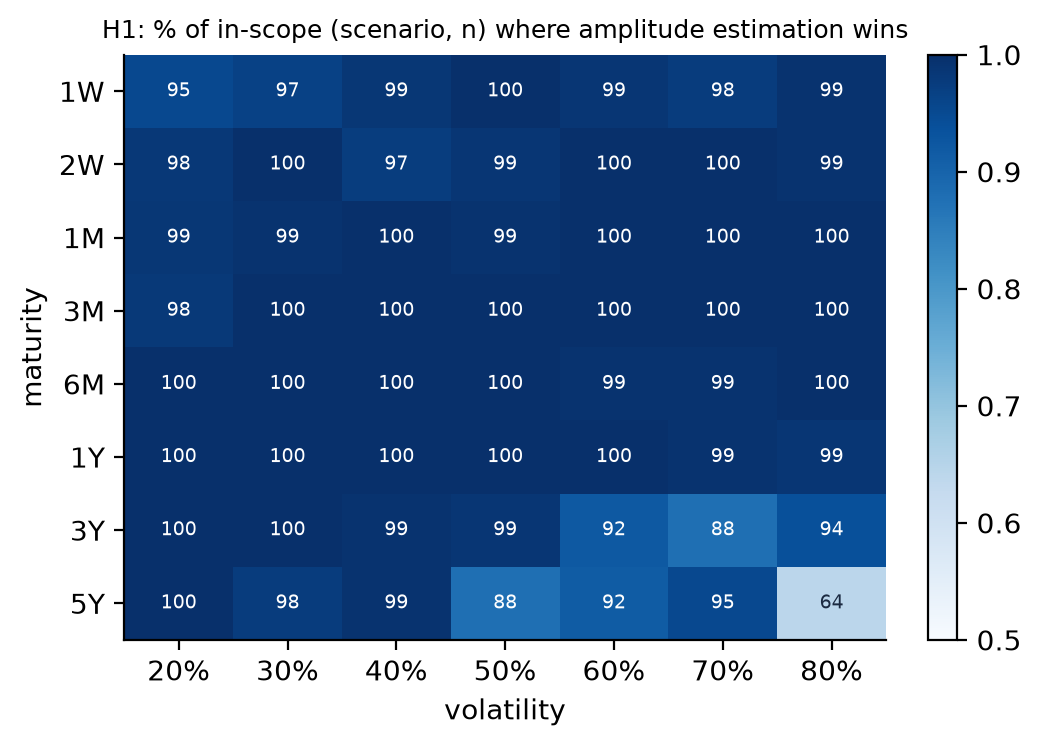
\includegraphics{img/h1_heatmap.png}

\textbf{Where it loses} {[}\texttt{H1\_failures}{]}: mostly at long
maturity and high volatility.

\begin{itemize}
\tightlist
\item
  Of the 191 losses, 106 are at 5Y and 46 at 3Y, and 73 are at 80\%
  volatility.
\item
  Losses grow with n: 14 at n = 3, 63 at n = 7.
\end{itemize}

\textbf{Why.} The price is read as e\^{}(−rT) × largest grid payoff ×
amplitude (Document 1, section 11). On a wide grid the largest payoff is
many times the price, so the amplitude is small and its error is
magnified. Monte Carlo on the grid has no such factor. Mode errors are
present in 37 of the 191 losses.

\textbf{When amplitude estimation gets ahead (n = 5)}
{[}\texttt{crossing\_budget\_n5},
\texttt{wins\_from\_budget\_onwards\_n5}{]}:

\begin{longtable}[]{@{}
  >{\raggedright\arraybackslash}p{(\columnwidth - 12\tabcolsep) * \real{0.3398}}
  >{\raggedright\arraybackslash}p{(\columnwidth - 12\tabcolsep) * \real{0.1034}}
  >{\raggedright\arraybackslash}p{(\columnwidth - 12\tabcolsep) * \real{0.1034}}
  >{\raggedright\arraybackslash}p{(\columnwidth - 12\tabcolsep) * \real{0.1034}}
  >{\raggedright\arraybackslash}p{(\columnwidth - 12\tabcolsep) * \real{0.1133}}
  >{\raggedright\arraybackslash}p{(\columnwidth - 12\tabcolsep) * \real{0.1133}}
  >{\raggedright\arraybackslash}p{(\columnwidth - 12\tabcolsep) * \real{0.1034}}@{}}
\toprule\noalign{}
\begin{minipage}[b]{\linewidth}\raggedright
Budget (calls)
\end{minipage} & \begin{minipage}[b]{\linewidth}\raggedright
1,800
\end{minipage} & \begin{minipage}[b]{\linewidth}\raggedright
3,500
\end{minipage} & \begin{minipage}[b]{\linewidth}\raggedright
6,800
\end{minipage} & \begin{minipage}[b]{\linewidth}\raggedright
13,300
\end{minipage} & \begin{minipage}[b]{\linewidth}\raggedright
26,200
\end{minipage} & \begin{minipage}[b]{\linewidth}\raggedright
Never
\end{minipage} \\
\midrule\noalign{}
\endhead
\bottomrule\noalign{}
\endlastfoot
First budget where it wins & 764 & 708 & 250 & 55 & 14 & 2 \\
First budget from which it wins at every larger budget & 657 & 637 & 297
& 119 & 50 & 33 \\
\end{longtable}

\begin{itemize}
\tightlist
\item
  82\% of scenarios have a first win by 3,500 calls.
\item
  72\% win at every budget from 3,500 onwards.
\end{itemize}

\hypertarget{26-h2-convergence-rate}{%
\subsubsection{2.6 H2: convergence rate}\label{26-h2-convergence-rate}}

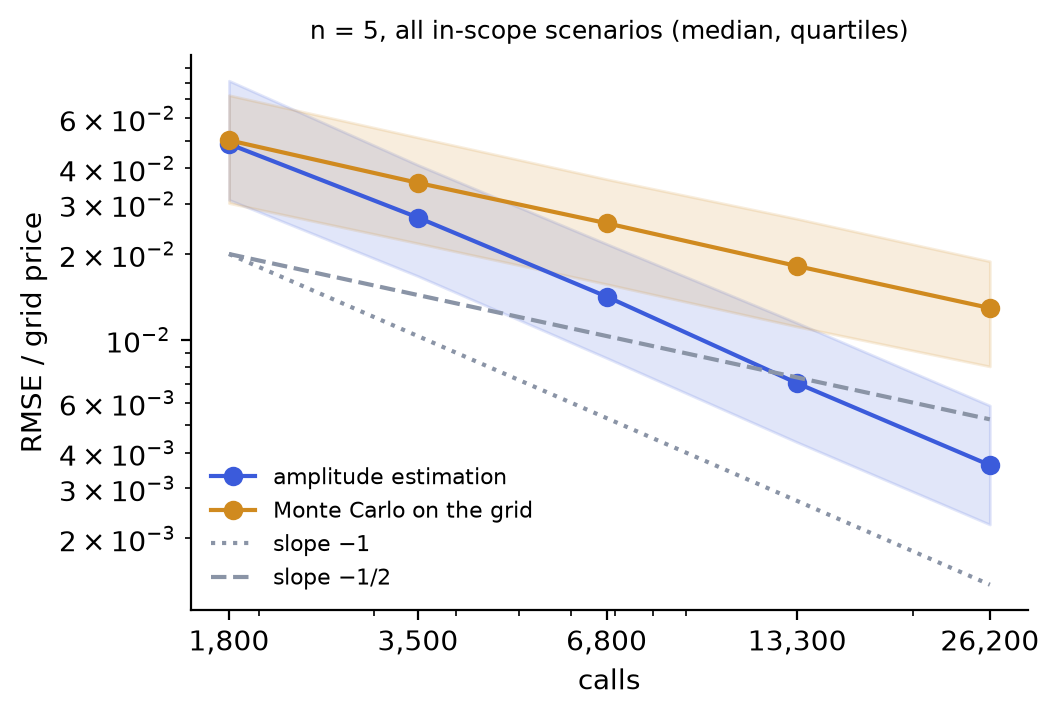
\includegraphics{img/error_vs_calls.png}

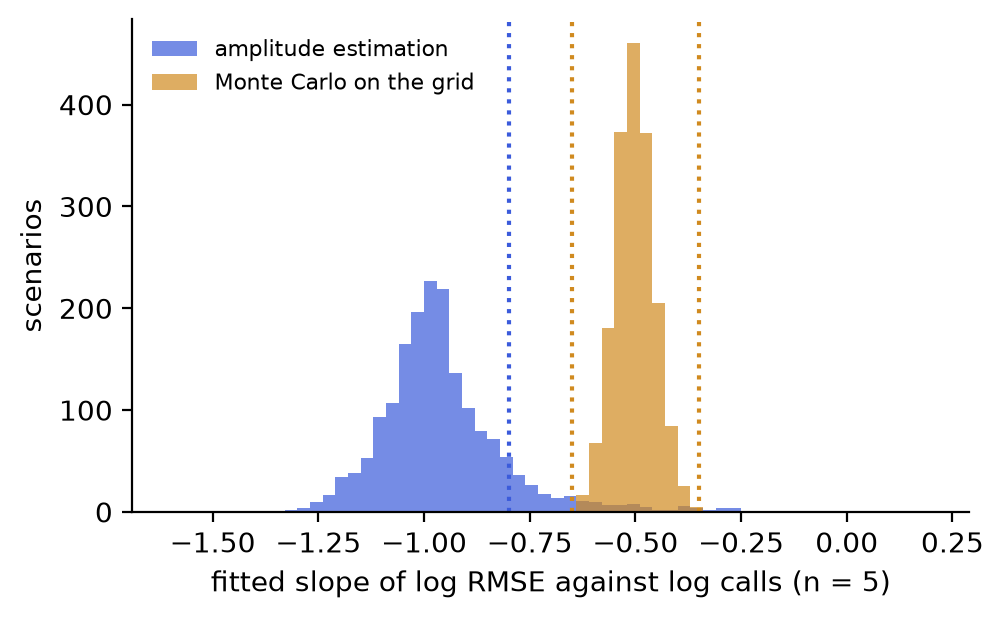
\includegraphics{img/slopes.png}

\textbf{Monte Carlo on the grid (H2-b) behaves as theory predicts.} The
median slope is −0.50, with quartiles −0.53 and −0.47, and 99.8\% of
scenarios fall in the band. This confirms both the benchmark and the
fitting procedure.

\textbf{Amplitude estimation (H2-a) shows the 1/N rate in the bulk of
scenarios.} The median slope is −0.98, with quartiles −1.04 and −0.90.
But 11.0\% of scenarios have a slope above −0.8, against the 10\% the
criterion allows.

\textbf{The limits rule, applied to H2-a and H3 alike.} Section 1.7
allows \emph{Validated with limits} "if a criterion fails only in an
identifiable region of the grid". The plan does not define "identifiable
region", so any region is chosen after seeing the results. Both
hypotheses are reported the same way {[}\texttt{H2a\_by\_maturity},
\texttt{H3\_by\_maturity}{]}:

\begin{longtable}[]{@{}
  >{\raggedright\arraybackslash}p{(\columnwidth - 8\tabcolsep) * \real{0.1707}}
  >{\raggedright\arraybackslash}p{(\columnwidth - 8\tabcolsep) * \real{0.2337}}
  >{\raggedright\arraybackslash}p{(\columnwidth - 8\tabcolsep) * \real{0.1653}}
  >{\raggedright\arraybackslash}p{(\columnwidth - 8\tabcolsep) * \real{0.1653}}
  >{\raggedright\arraybackslash}p{(\columnwidth - 8\tabcolsep) * \real{0.2451}}@{}}
\toprule\noalign{}
\begin{minipage}[b]{\linewidth}\raggedright
\end{minipage} & \begin{minipage}[b]{\linewidth}\raggedright
Pass rate, maturities 1W to 1Y
\end{minipage} & \begin{minipage}[b]{\linewidth}\raggedright
Pass rate at 3Y
\end{minipage} & \begin{minipage}[b]{\linewidth}\raggedright
Pass rate at 5Y
\end{minipage} & \begin{minipage}[b]{\linewidth}\raggedright
Restricted to maturities up to 1Y
\end{minipage} \\
\midrule\noalign{}
\endhead
\bottomrule\noalign{}
\endlastfoot
H2-a (needs 90\%) & 88\% to 93\% & 84\% & 81\% & 91.2\%: passes \\
H3 (needs 95\%) & 98\% to 100\% & 70\% & 50\% & 99.0\%: passes \\
\end{longtable}

\begin{itemize}
\tightlist
\item
  \textbf{H3 failures are concentrated:} 185 of the 198 failures are at
  3Y and 5Y, and every maturity up to 1Y passes on its own.
\item
  \textbf{H2-a failures are spread out:} they appear at every maturity
  and every volatility. Pass rates by volatility run from 85\% to 91\%,
  and two maturities within the "up to 1Y" region fail on their own (3M
  at 88.3\%, 1Y at 89.6\%). Restricting to maturities up to 1Y lifts
  H2-a just above 90\% by averaging, not by removing the failures.
\end{itemize}

\textbf{The developer\textquotesingle s reading:}

\begin{itemize}
\tightlist
\item
  H3 is \emph{Validated with limits} (maturities up to 1 year);
\item
  H2-a is \emph{Not validated}.
\end{itemize}

This reading treats "only in an identifiable region" as requiring the
criterion to hold for each maturity inside the region. That condition is
not in the plan, so the reading is a judgement. It is left to the review
and the sign-off.

\textbf{Likely reasons for the H2-a dispersion (not tested):}

\begin{itemize}
\tightlist
\item
  \textbf{Noise in each slope.} Each slope is fitted on 5 RMSEs, each
  estimated from 50 draws, so each RMSE carries a relative standard
  error of about 10\%. Over this range of budgets, that moves the slope
  by several hundredths.
\item
  \textbf{The low budgets are not asymptotic.} At depth 4 (powers 0, 1
  and 2 only), MLAE is not yet in its asymptotic regime, so the fitted
  slope mixes two regimes.
\item
  \textbf{Follow-ups.} A longer ladder or more draws would sharpen the
  estimate. Neither was planned.
\end{itemize}

\hypertarget{27-h3-accuracy-against-black-scholes-n--7}{%
\subsubsection{2.7 H3: accuracy against Black-Scholes, n =
7}\label{27-h3-accuracy-against-black-scholes-n--7}}

Against Black-Scholes, the RMSE is within max(1\% of the price, 0.01) in
89.0\% of scenarios overall, and in \textbf{99.0\%} of the 1,331
scenarios with maturity up to 1 year {[}\texttt{H3},
\texttt{H3\_up\_to\_1Y}{]}. Failures grow with volatility: 70 of them
are at 80\% {[}\texttt{H3\_failures}{]}.

\textbf{Two causes:}

\begin{itemize}
\tightlist
\item
  \textbf{Discretisation bias, in 67 of the 198 failures.} There, the
  bias alone exceeds the tolerance: no amount of sampling can bring
  those scenarios within 1\% with 128 grid points.
\item
  \textbf{The payoff scaling described in 2.5,} in the rest.
\end{itemize}

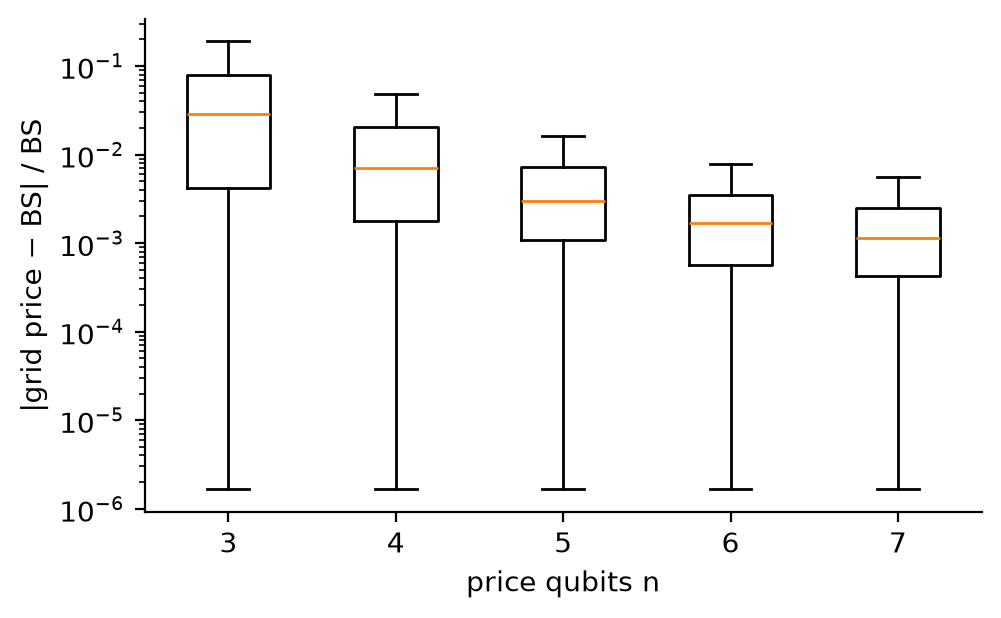
\includegraphics{img/discretisation_bias.png}

The median relative discretisation bias falls from 2.9\% at n = 3 to
0.11\% at n = 7 {[}\texttt{discretisation\_bias\_rel}{]}.

\hypertarget{28-h4-and-relative-efficiency}{%
\subsubsection{2.8 H4 and relative
efficiency}\label{28-h4-and-relative-efficiency}}

\textbf{Against quasi-Monte Carlo} (n = 7, both against Black-Scholes),
amplitude estimation\textquotesingle s RMSE is a median \textbf{18 to 20
times larger}, at every budget {[}\texttt{H4\_ratio\_qae\_over\_qmc}{]}.
Amplitude estimation has the lower RMSE in only 4 to 9 of the 1,793
scenarios, depending on the budget {[}\texttt{H4\_qae\_wins}{]}.

\begin{itemize}
\tightlist
\item
  The ratio is roughly constant across budgets, so both methods converge
  at about the same rate, as stated in advance.
\item
  The constant favours quasi-Monte Carlo, because amplitude estimation
  carries the discretisation bias and the payoff scaling, and
  quasi-Monte Carlo carries neither.
\end{itemize}

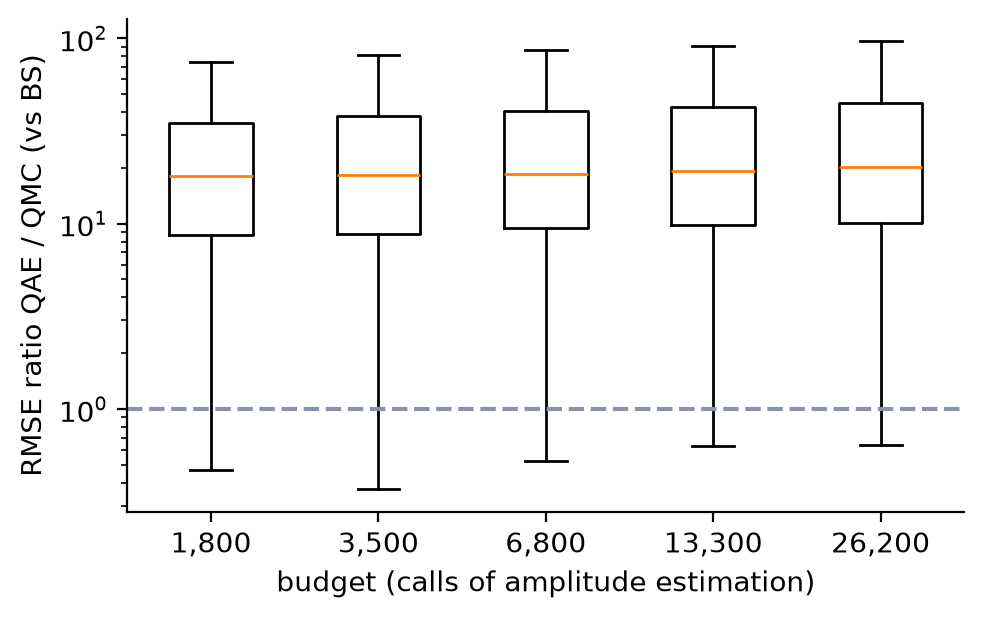
\includegraphics{img/qae_vs_qmc.png}

\textbf{Relative efficiency at the largest budget}, E = N\_comparator(ε)
/ N\_QAE(ε) {[}\texttt{relative\_efficiency\_largest\_budget}{]}:

\begin{longtable}[]{@{}
  >{\raggedright\arraybackslash}p{(\columnwidth - 8\tabcolsep) * \real{0.2459}}
  >{\raggedright\arraybackslash}p{(\columnwidth - 8\tabcolsep) * \real{0.1211}}
  >{\raggedright\arraybackslash}p{(\columnwidth - 8\tabcolsep) * \real{0.1658}}
  >{\raggedright\arraybackslash}p{(\columnwidth - 8\tabcolsep) * \real{0.1602}}
  >{\raggedright\arraybackslash}p{(\columnwidth - 8\tabcolsep) * \real{0.2871}}@{}}
\toprule\noalign{}
\begin{minipage}[b]{\linewidth}\raggedright
Comparison
\end{minipage} & \begin{minipage}[b]{\linewidth}\raggedright
Median E
\end{minipage} & \begin{minipage}[b]{\linewidth}\raggedright
Quartiles
\end{minipage} & \begin{minipage}[b]{\linewidth}\raggedright
E \textgreater{} 1
\end{minipage} & \begin{minipage}[b]{\linewidth}\raggedright
Comparator\textquotesingle s N(ε) outside the budgets run
\end{minipage} \\
\midrule\noalign{}
\endhead
\bottomrule\noalign{}
\endlastfoot
vs Monte Carlo on the grid, n = 5 & 11.2 & 6.7 -- 18.1 & 1,759 of 1,793
& above 26,200 calls in 1,759; below 1,800 in 2 \\
vs Monte Carlo on the grid, n = 7 & 10.4 & 6.0 -- 17.3 & 1,732 of 1,793
& above 26,200 calls in 1,732 \\
vs quasi-Monte Carlo, n = 7 & 0.028 & 0.014 -- 0.050 & 2 of 1,793 &
below 1,024 points in 1,155; above in 3 \\
\end{longtable}

At the largest budget, plain Monte Carlo would need about \textbf{11
times more calls} than amplitude estimation to reach the same error on
the grid. Quasi-Monte Carlo would need about \textbf{36 times fewer}.

Both figures come from extrapolating each comparator\textquotesingle s
fitted line outside the budgets actually run, in almost every scenario.
They are indicative, not measured.

\hypertarget{29-mode-errors-of-mlae}{%
\subsubsection{2.9 Mode errors of MLAE}\label{29-mode-errors-of-mlae}}

\textbf{Mode errors are rare} {[}\texttt{mode\_errors}{]}:

\begin{longtable}[]{@{}
  >{\raggedright\arraybackslash}p{(\columnwidth - 6\tabcolsep) * \real{0.3809}}
  >{\raggedright\arraybackslash}p{(\columnwidth - 6\tabcolsep) * \real{0.2428}}
  >{\raggedright\arraybackslash}p{(\columnwidth - 6\tabcolsep) * \real{0.1782}}
  >{\raggedright\arraybackslash}p{(\columnwidth - 6\tabcolsep) * \real{0.1782}}@{}}
\toprule\noalign{}
\begin{minipage}[b]{\linewidth}\raggedright
\end{minipage} & \begin{minipage}[b]{\linewidth}\raggedright
Depths 4 to 6
\end{minipage} & \begin{minipage}[b]{\linewidth}\raggedright
Depth 7
\end{minipage} & \begin{minipage}[b]{\linewidth}\raggedright
Depth 8
\end{minipage} \\
\midrule\noalign{}
\endhead
\bottomrule\noalign{}
\endlastfoot
Share of draws affected & 0\% & 0.0007\% & 0.009\% \\
Configurations with at least one & 0 of 8,965 & 3 & 40 \\
\end{longtable}

The 0\% at depths 4 to 6 is partly a consequence of the definition: the
threshold is wider for short ladders (Document 1, section 6).

\textbf{They come from the method, not the optimiser.} For all 43
configurations with a mode error, the draws were regenerated from their
seeds and compared with a 400,001-point grid. The estimator agrees with
the fine grid in all 2,150 draws
{[}\texttt{checks.json:\ mlae\_global\_maximum}{]}.

\textbf{A single one can still dominate an RMSE.} Mode errors are
present in 37 of the 191 H1 losses. The scenario that revealed them
(section 1.9) is among the 40 at depth 8.

\hypertarget{210-conclusions}{%
\subsubsection{2.10 Conclusions}\label{210-conclusions}}

These conclusions hold \textbf{if the restatement of H0-a in 2.4 is
accepted}. Without it, the plan gives no verdict on H1 to H4.

\begin{enumerate}
\def\labelenumi{\arabic{enumi}.}
\tightlist
\item
  \textbf{The circuit does what it claims, up to numerical precision.}

  \begin{itemize}
  \tightlist
  \item
    It reproduces the grid price to a relative 3.4e-9.
  \item
    The Grover identity behind the fast simulation holds to 6.1e-10, up
    to the largest power used.
  \item
    H0-a failed as written because its absolute tolerance was too tight
    for 7-qubit synthesis, not because of an error in the circuit.
  \end{itemize}
\item
  \textbf{Amplitude estimation beats plain Monte Carlo at equal calls on
  the same grid, at the budgets tested.} It does so in 97.9\% of cases
  at 26,200 calls. This is the advantage measured. The quadratic rate
  behind the textbook claim is seen in the bulk (median slope −0.98) but
  \textbf{not certified} at the planned threshold (conclusion 3). The
  figure of 11 times fewer calls is extrapolated.
\item
  \textbf{The 1/N rate is not certified scenario by scenario.} 11\% of
  scenarios have a fitted slope above −0.8, against 10\% allowed, and
  they are not confined to one region.
\item
  \textbf{Against Black-Scholes, the kit is accurate to 1\% for
  maturities up to 1 year} with 7 price qubits. Beyond that, both the
  discretisation and the payoff scaling degrade it.
\item
  \textbf{There is no gain over the best classical sampler.} Quasi-Monte
  Carlo is about 20 times more accurate at the same budget on this
  one-dimensional problem. That was expected, and it is why a European
  call is a test bench, not a use case.
\end{enumerate}

\hypertarget{211-overall-verdict-developer}{%
\subsubsection{2.11 Overall verdict
(developer)}\label{211-overall-verdict-developer}}

The stated purpose is a reproducible, documented test bench for
amplitude estimation on the simplest option. \textbf{For that purpose,
the kit is fit, with limits, conditional on accepting the restatement of
H0-a.}

\begin{longtable}[]{@{}
  >{\raggedright\arraybackslash}p{(\columnwidth - 2\tabcolsep) * \real{0.4472}}
  >{\raggedright\arraybackslash}p{(\columnwidth - 2\tabcolsep) * \real{0.5328}}@{}}
\toprule\noalign{}
\begin{minipage}[b]{\linewidth}\raggedright
Point
\end{minipage} & \begin{minipage}[b]{\linewidth}\raggedright
Status
\end{minipage} \\
\midrule\noalign{}
\endhead
\bottomrule\noalign{}
\endlastfoot
Correctness of the circuit and the simulation & Established up to
numerical precision; the restatement of H0-a is needed for the
plan\textquotesingle s criterion to pass \\
Fewer calls than plain Monte Carlo on the same grid, at the budgets
tested & Established (H1), conditional on H0-a \\
The 1/N rate, scenario by scenario at the planned threshold & Not
established (H2-a) \\
Accuracy against Black-Scholes & Up to 1 year only (H3), conditional on
H0-a \\
Advantage over quasi-Monte Carlo & None, as expected \\
\end{longtable}

\textbf{For the independent review and the sign-off to decide:}

\begin{enumerate}
\def\labelenumi{\arabic{enumi}.}
\tightlist
\item
  Accept or reject the restatement of H0-a.
\item
  Accept or reject the developer\textquotesingle s reading of the limits
  rule for H2-a and H3.
\item
  Decide whether H2-a calls for a follow-up campaign: a longer ladder,
  more draws, or both.
\end{enumerate}

\end{document}
